\section{Aprendizaje supervisado: regresión logística}
\label{sec:punto1}

% Punto 1 (60 puntos). Archivo: src/tp2/punto1.py. Pruebas: tests/test_punto1.py.

\subsection{Evaluación del modelo}

La regresión logística modela la probabilidad de que un mensaje sea spam como
\[
    p(y=1\mid x) = \sigma(x^\top w + b), \qquad \sigma(z) = \frac{1}{1+e^{-z}}.
\]
La función \texttt{forward} es una implementación propia en PyTorch
\cite{paszke2019pytorch}, sin \texttt{torch.nn}. Calcula los logits
$z = Xw + b$ de las $n$ muestras con un único producto matriz-vector y les
aplica la sigmoide. Para que la sigmoide no se desborde con logits grandes,
se evalúa con $e^{-|z|}\in(0,1]$:
\[
    \sigma(z) =
    \begin{cases}
        \dfrac{1}{1+e^{-|z|}} & z \geq 0,\\[2ex]
        \dfrac{e^{-|z|}}{1+e^{-|z|}} & z < 0.
    \end{cases}
\]
Ninguna de las dos ramas produce infinitos, ni en el valor ni en el
gradiente, mientras que la forma directa $1/(1+e^{-z})$ calcula $e^{1000}$
para $z=-1000$ y su gradiente con Autograd resulta indefinido.

\subsection{Entrenamiento}

La función \texttt{train\_logistic\_regression} minimiza la entropía cruzada
binaria media
\[
    L(w,b) = -\frac{1}{n}\sum_{i=1}^{n}
    \left[y_i\log p_i + (1-y_i)\log(1-p_i)\right],
    \qquad p_i = \sigma(x_i^\top w + b),
\]
con descenso del gradiente por lotes completos, también implementado sin
optimizadores de PyTorch. En cada época se evalúa $p$ con \texttt{forward} y
se aplica el gradiente exacto de $L$:
\[
    w \leftarrow w - \frac{\alpha}{n} X^\top (p - y), \qquad
    b \leftarrow b - \frac{\alpha}{n} \sum_{i=1}^{n} (p_i - y_i).
\]
Los pesos se inicializan con una normal de desviación $0.01$ generada con la
semilla de la corrida y el sesgo, en cero, de modo que la misma semilla
reproduce el mismo modelo. El entrenamiento ejecuta un número fijo de épocas
con una tasa de aprendizaje $\alpha$ fija: $\alpha=0.1$ y 1000 épocas en los
datos sintéticos, y $\alpha=10$ y 2000 épocas, calibrados en la
Sección~\ref{sec:calibracion}, sobre los mensajes. El historial de pérdida
guarda la pérdida inicial y la de cada época, calculada como
$\log(1+e^{z_i}) - y_i z_i$, expresión equivalente a la entropía cruzada que
no se indefine cuando $p_i$ vale exactamente 0 o 1.

\subsection{Verificación con datos linealmente separables}
\label{sec:sinteticos}

Antes de usar los mensajes, se verifica el regresor en un caso donde la
respuesta correcta se conoce. La frontera verdadera es la recta
\[
    w^{*\top}x + b^* = 0.6\,x_1 + 0.8\,x_2 - 0.5 = 0 .
\]
Como $\lVert w^*\rVert = 1$, $w^{*\top}x+b^*$ es la distancia con signo de
$x$ a la recta. Cada punto se coloca a una distancia
$|d| = 1 + 0.5\,|z|$, con $z\sim\mathcal{N}(0,1)$, del lado de su clase (la
clase 1 donde $d>0$) y a una posición $\mathcal{N}(0, 2^2)$ a lo largo de la
recta. Entre las dos clases queda una franja vacía de ancho 2, así que los
datos son linealmente separables por construcción. Se generan 200 puntos de
entrenamiento (100 por clase) y otros 200 de prueba con otra semilla
(Figura~\ref{fig:sinteticos-datos}).

\begin{figure}[H]
    \centering
    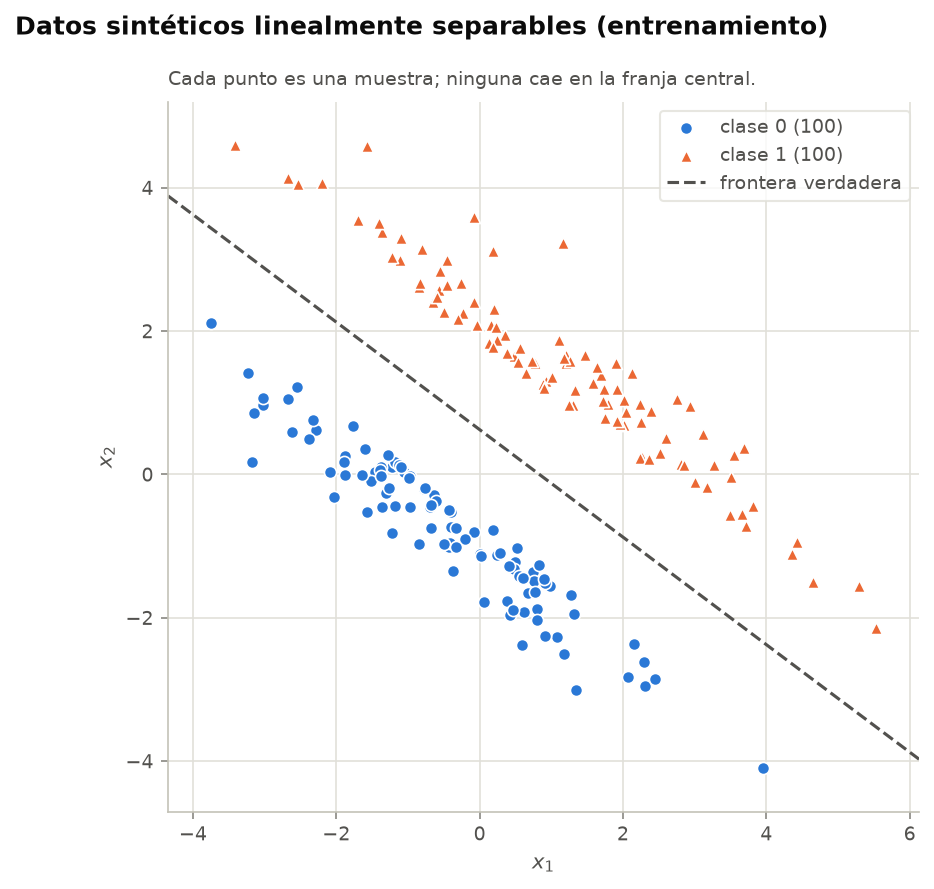
\includegraphics[width=0.62\textwidth]{datos-sinteticos-linealmente-separables-entrenamiento}
    \caption{Datos sintéticos de entrenamiento y frontera verdadera.}
    \label{fig:sinteticos-datos}
\end{figure}

El modelo se entrena con $\alpha=0.1$ durante 1000 épocas. Como el
entrenamiento es determinista para una semilla dada, entrenar $k$ épocas
reproduce exactamente el estado del entrenamiento completo en la época $k$;
así se obtienen las fronteras intermedias de la
Figura~\ref{fig:sinteticos-proceso}. La Tabla~\ref{tab:sinteticos-evolucion}
compara cada estado con la frontera verdadera: como la recta $w^\top x+b=0$
no cambia al multiplicar $w$ y $b$ por una constante, se reportan $w$ y $b$
divididos por $\lVert w\rVert$ y el ángulo entre $w$ y $w^*$.

\begin{figure}[H]
    \centering
    \begin{subfigure}{0.49\textwidth}
        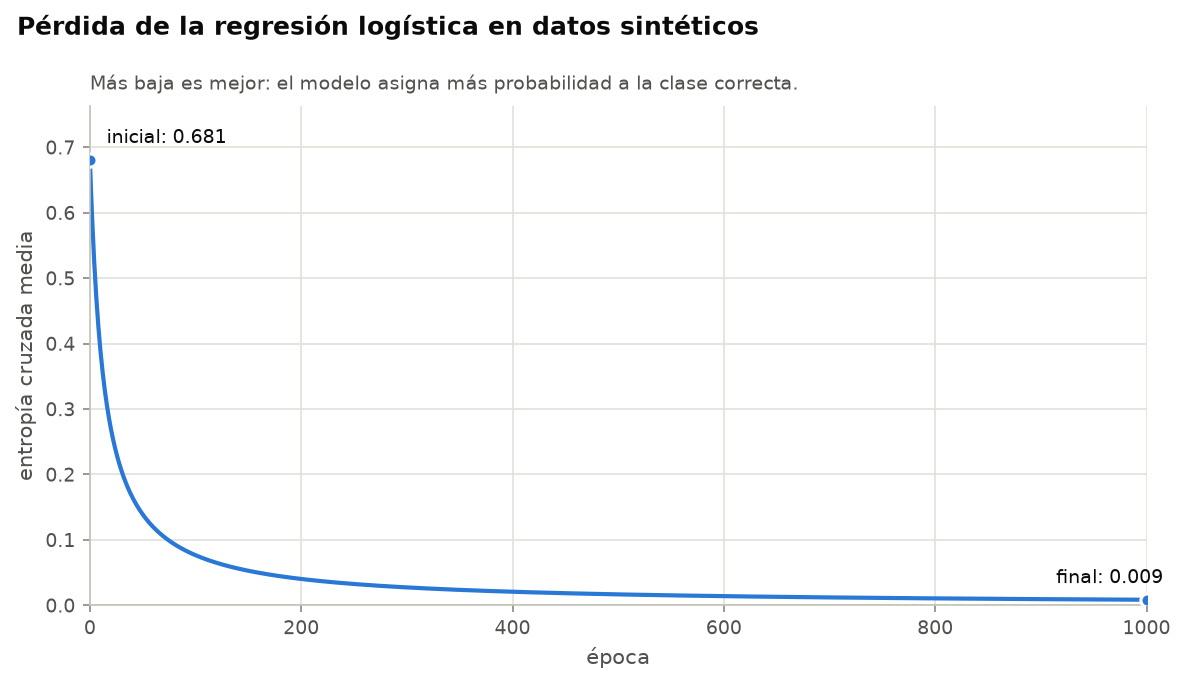
\includegraphics[width=\linewidth]{perdida-de-la-regresion-logistica-en-datos-sinteticos}
        \caption{Entropía cruzada media en cada época.}
    \end{subfigure}
    \hfill
    \begin{subfigure}{0.49\textwidth}
        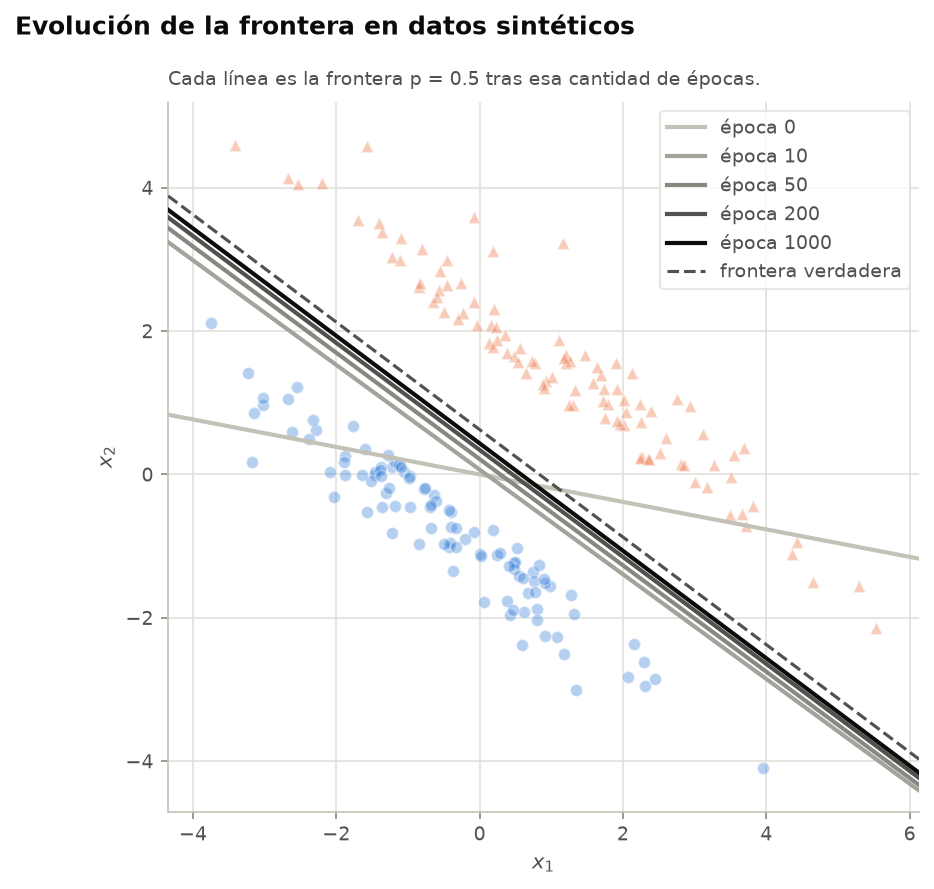
\includegraphics[width=\linewidth]{evolucion-de-la-frontera-en-datos-sinteticos}
        \caption{Frontera $p=0.5$ tras 0, 10, 50, 200 y 1000 épocas.}
    \end{subfigure}
    \caption{Proceso de entrenamiento sobre los datos sintéticos.}
    \label{fig:sinteticos-proceso}
\end{figure}

\begin{table}[H]
    \centering
    \caption{Evolución del entrenamiento en datos sintéticos.}
    \label{tab:sinteticos-evolucion}
    \small
    \begin{tabular}{rcccccc}
        \toprule
        Época & Pérdida & Aciertos (entr.) & $w_1/\lVert w\rVert$ & $w_2/\lVert w\rVert$ & $b/\lVert w\rVert$ & Ángulo con $w^*$ \\
        \midrule
        0    & 0.681 & 0.90 & 0.188 & 0.982 & 0.000  & 26.02° \\
        10   & 0.388 & 1.00 & 0.590 & 0.808 & $-0.054$ & 0.73° \\
        50   & 0.139 & 1.00 & 0.596 & 0.803 & $-0.172$ & 0.31° \\
        200  & 0.040 & 1.00 & 0.598 & 0.801 & $-0.274$ & 0.13° \\
        1000 & 0.009 & 1.00 & 0.600 & 0.800 & $-0.347$ & 0.01° \\
        \midrule
        Verdadera & --- & --- & 0.600 & 0.800 & $-0.500$ & 0° \\
        \bottomrule
    \end{tabular}
\end{table}

\begin{figure}[H]
    \centering
    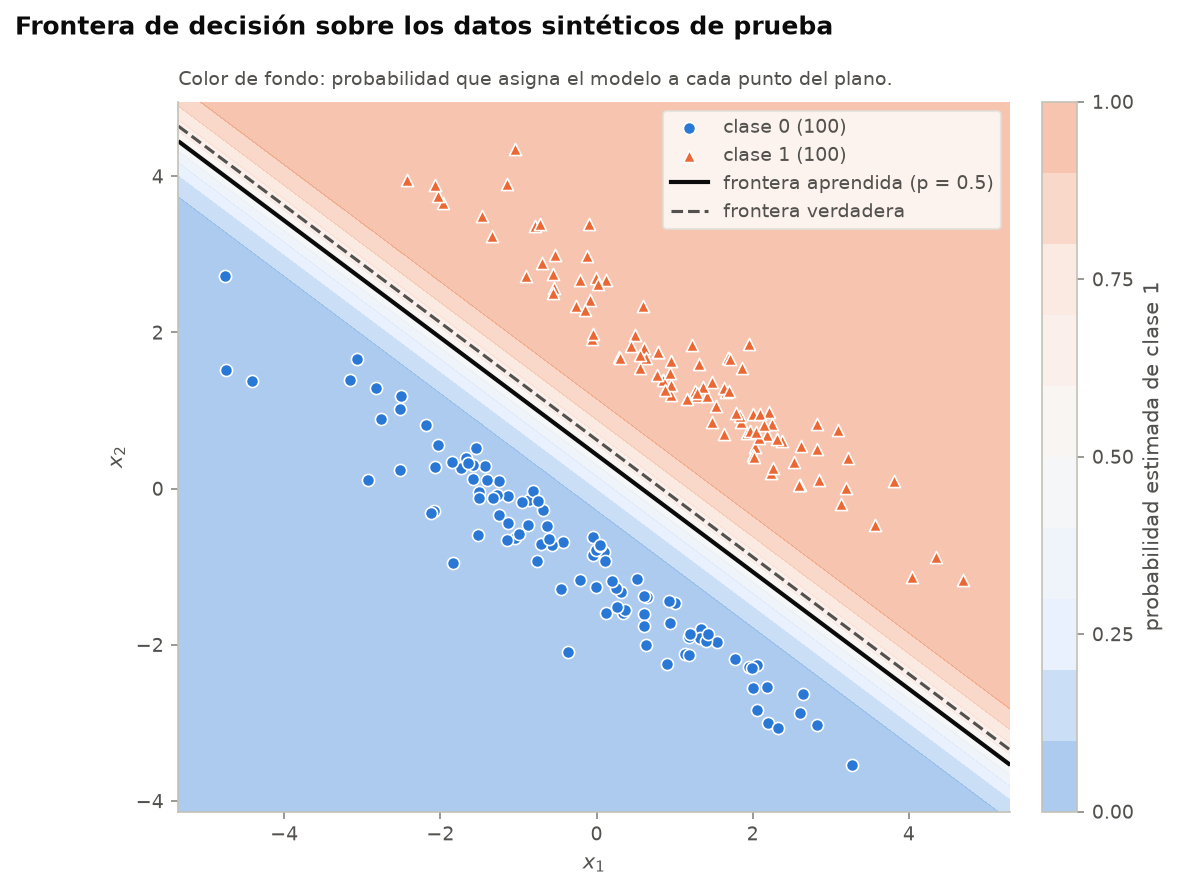
\includegraphics[width=0.7\textwidth]{frontera-de-decision-sobre-los-datos-sinteticos-de-prueba}
    \caption{Probabilidad estimada por el modelo final y frontera aprendida
    sobre los 200 puntos de prueba.}
    \label{fig:sinteticos-frontera}
\end{figure}

El regresor recupera la frontera verdadera. En la época 0 los pesos son casi
nulos ($\lVert w\rVert=0.02$) y la frontera está girada 26° respecto de la
verdadera; tras 10 épocas ya clasifica bien todo el entrenamiento y tras 1000
el ángulo es de 0.01°. La pérdida baja de 0.681 a 0.009 sin oscilar. En los
200 puntos de prueba la tasa de aciertos y el F1-score valen 1
(Figura~\ref{fig:sinteticos-frontera}).

Dos detalles muestran cómo aprende la regresión logística con datos
separables. Primero, $\lVert w\rVert$ crece sin parar (de 0.02 a 3.84): como
existe una recta que separa todo, la pérdida se puede seguir reduciendo
haciendo más abrupta la transición de probabilidad, sin cambiar la recta; por
eso la franja de colores alrededor de la frontera es angosta. Segundo, el
sesgo normalizado ($-0.35$) todavía no alcanza el verdadero ($-0.5$): la
frontera aprendida está desplazada 0.15 hacia la clase 0, pero dentro de la
franja vacía, así que clasifica todo bien. Con datos separables hay infinitas
rectas que separan perfectamente, y el descenso del gradiente se mueve muy
lentamente hacia la de margen máximo \cite{soudry2018implicit}: la
orientación converge mucho antes que la posición.

\subsection{Extracción de características y clasificación}
\label{sec:caracteristicas}

\paragraph{Codificador.} Cada mensaje, sin preprocesar, se convierte en un
vector con \texttt{all-MiniLM-L6-v2}, un modelo de la biblioteca
sentence-transformers \cite{reimers2019sentence} basado en MiniLM
\cite{wang2020minilm} y entrenado para que oraciones de significado parecido
queden cerca. Produce vectores de $D=384$ dimensiones con norma 1. Se eligió
frente a BERT base y DistilBERT porque está pensado para representar
oraciones completas y codifica los 5\,574 mensajes en CPU en poco tiempo. Las
características se calculan una sola vez y se guardan, porque no dependen de
la partición.

\paragraph{Calibración.}
\label{sec:calibracion}
Con vectores de norma 1, cada coordenada vale del orden de
$1/\sqrt{384}\approx0.05$ y el gradiente es pequeño: con $\alpha=0.1$ y
1000 épocas, los valores de la Sección~\ref{sec:sinteticos}, el modelo casi
no aprende (en una ejecución preliminar, el F1 medio de las 30 corridas fue
0.23). Para elegir $\alpha$ y las épocas sin usar la prueba, se tomó el
70~\% de entrenamiento de la primera partición y se separó de él un 20~\%
estratificado como validación (781 mensajes, 105 de ellos spam). Con el 80~\%
restante se entrenó cada combinación de
$\alpha\in\{0.5,1,2,5,10,20,50\}$ y $\{250,500,1000,2000,4000\}$ épocas, y
se eligió la de mayor F1 en la validación. Como el F1 de una validación con
105 spam cambia a saltos, varias combinaciones empatan; el empate se resolvió
con la menor entropía cruzada en la validación
(Figura~\ref{fig:calibracion}).

\begin{figure}[H]
    \centering
    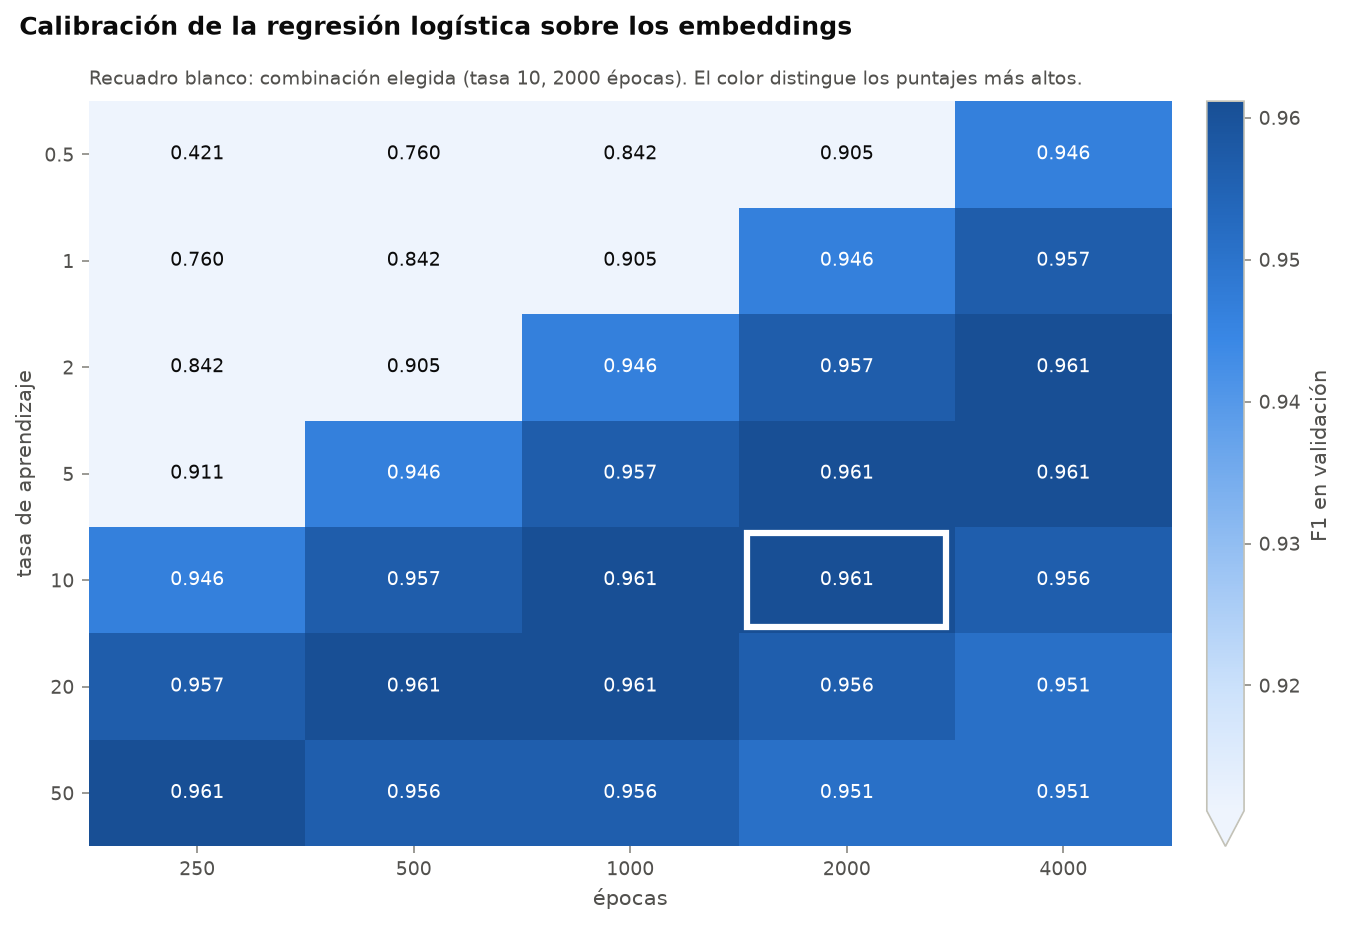
\includegraphics[width=0.85\textwidth]{calibracion-de-la-regresion-logistica-sobre-los-embeddings}
    \caption{F1 en la validación para cada combinación de tasa de
    aprendizaje y épocas.}
    \label{fig:calibracion}
\end{figure}

Lo que importa es el producto $\alpha\times$épocas: $10\times2000$,
$5\times4000$ y $20\times1000$ (todas 20\,000) dan el mismo F1 de validación
(0.961) y casi la misma pérdida (0.0463). Con poco entrenamiento el F1 cae a
0.42 ($0.5\times250$); con demasiado ($50\times4000$) la pérdida de ajuste
sigue bajando (0.004), pero la de validación sube (0.059) y el F1 baja a
0.951, una señal leve de sobreajuste. Se eligieron $\alpha=10$ y 2000 épocas.

\paragraph{Resultados de las 30 corridas.} Cada corrida usa una partición
estratificada 70/30 distinta, entrena con los valores calibrados y evalúa en
su prueba de 1\,672 mensajes (1\,448 ham y 224 spam). La
Tabla~\ref{tab:resultados-rl} resume las métricas y la
Figura~\ref{fig:resultados-rl} muestra cada corrida y la matriz de confusión
promedio.

\begin{table}[H]
    \centering
    \caption{Regresión logística sobre las características del codificador
    (30 corridas).}
    \label{tab:resultados-rl}
    \begin{tabular}{lcccc}
        \toprule
        Métrica & Media & Desviación & Mínimo & Máximo \\
        \midrule
        Tasa de aciertos & 0.9876 & 0.0022 & 0.9839 & 0.9916 \\
        F1-score         & 0.9528 & 0.0084 & 0.9388 & 0.9683 \\
        \bottomrule
    \end{tabular}
\end{table}

\begin{figure}[H]
    \centering
    \begin{subfigure}{0.52\textwidth}
        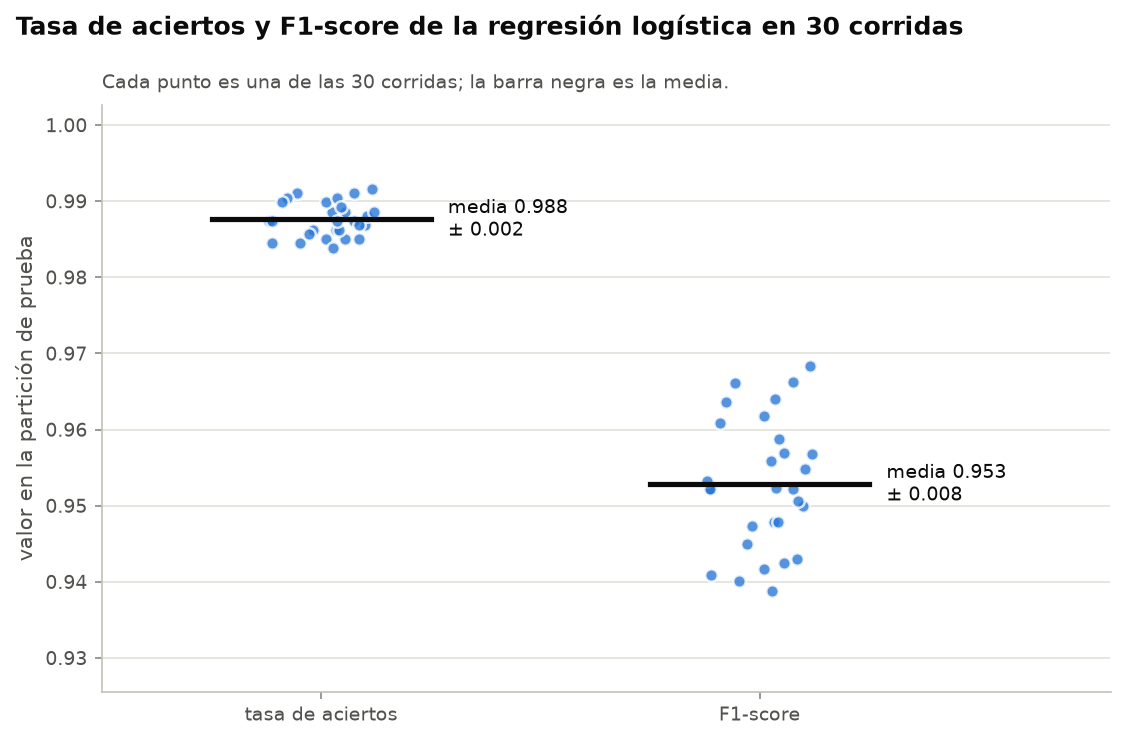
\includegraphics[width=\linewidth]{tasa-de-aciertos-y-f1-score-de-la-regresion-logistica-en-30-corridas}
        \caption{Métricas de cada corrida y su media.}
    \end{subfigure}
    \hfill
    \begin{subfigure}{0.44\textwidth}
        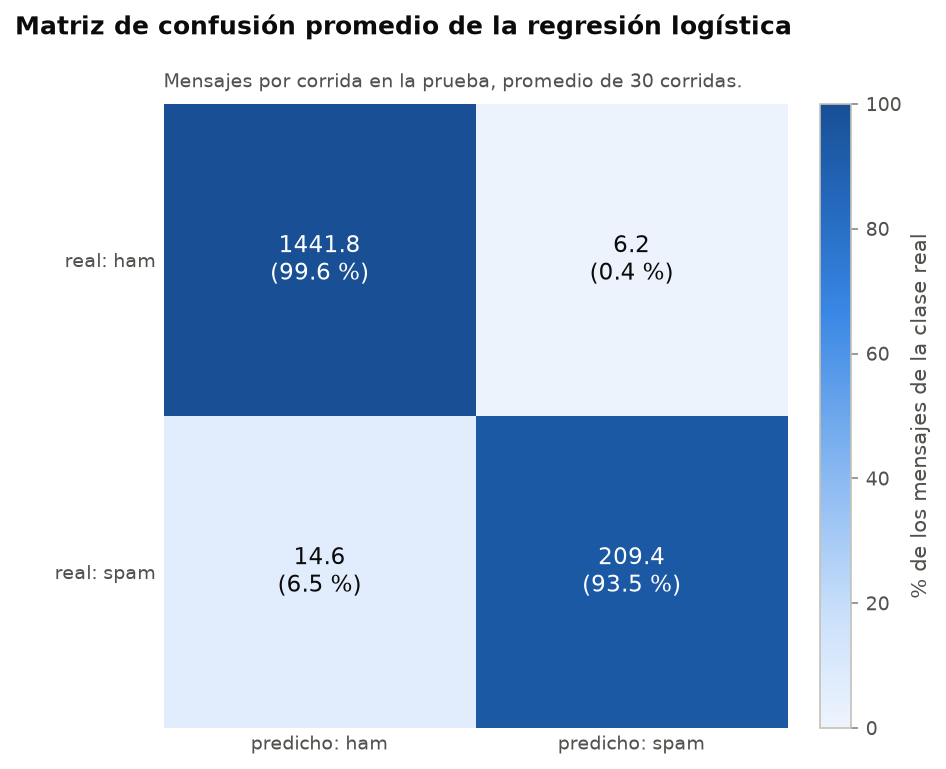
\includegraphics[width=\linewidth]{matriz-de-confusion-promedio-de-la-regresion-logistica}
        \caption{Matriz de confusión promedio.}
    \end{subfigure}
    \caption{Resultados de la regresión logística en las 30 corridas.}
    \label{fig:resultados-rl}
\end{figure}

La dispersión entre corridas es pequeña, así que el resultado no depende de
una partición afortunada. El F1 varía más que la tasa de aciertos porque solo
depende de los 224 spam de cada prueba: cada spam mal clasificado lo mueve
unas 0.0025. En promedio, de los 1\,448 ham solo 6.2 se marcan como spam
(0.4~\%), mientras que de los 224 spam se escapan 14.6 (6.5~\%): precisión
0.971 y exhaustividad 0.935. Casi todos los errores son spam que el modelo
deja pasar, el lado preferible para un filtro, porque perder un mensaje real
es peor que recibir un spam; bajar el umbral de 0.5 detectaría más spam a
costa de más falsas alarmas. Como referencia, un clasificador que respondiera
siempre ``ham'' tendría una tasa de aciertos de 0.866 y un F1 de 0.

Una limitación: la calibración usa datos de la primera partición que en otras
corridas pueden caer en la prueba. Solo se eligieron dos números con ellos,
así que el sesgo optimista es pequeño, pero existe.

\subsection{Reducción de dimensionalidad con PCA}

TODO (punto 1.5): describir el PCA, graficar el dataset reducido a 50~\%,
25~\% y 2 dimensiones, analizar la clasificación con regresión logística en
cada caso y justificar la $D$ óptima que usa el detector de anomalías.
